\chapter{DESIGN AND METHODOLOGY}

\section{Introduction}

This chapter presents the design and methodology of the proposed 
Machine Learning-based message prioritization and congestion-aware 
rate control system for UAV communication networks. The objective of 
the proposed system is to enhance communication reliability, reduce 
packet loss, and improve overall network performance in MAVLink-based 
UAV communication environments.

Modern UAV networks operate under dynamic conditions where multiple 
types of messages are transmitted simultaneously. Traditional 
communication systems rely on fixed transmission strategies, which 
may lead to congestion and inefficient bandwidth utilization. The 
proposed methodology integrates Machine Learning techniques with 
adaptive rate control mechanisms to intelligently manage network 
traffic.

The system is designed using a modular architecture in which each 
module performs a specific function. This modular approach enhances 
system scalability, flexibility, and maintainability, making it 
suitable for large-scale UAV deployments.

%-------------------------------------------------------------

\section{System Architecture}

The proposed system architecture consists of multiple functional 
modules that collectively improve communication efficiency in UAV 
networks. Each module performs a well-defined operation and passes 
processed information to the next module.

The system begins with message generation from UAV sensors and 
control systems. These messages are then processed using a Machine 
Learning-based classification model that assigns appropriate priority 
levels. Based on network conditions, transmission rates are adjusted 
to avoid congestion. Messages are finally scheduled and transmitted 
according to their priority.

The major functional components of the system include:

\begin{itemize}

\item Message Generation Module

\item Machine Learning-Based Message Classification Module

\item Congestion Estimation Module

\item Adaptive Rate Control Module consists of Priority Queue Scheduling methodology

\item Message Transmission Module.

\end{itemize}

These modules interact sequentially to ensure efficient handling 
of network traffic and reliable delivery of critical communication 
messages.

In the extended combined model used in this project, the system is 
implemented as a closed loop between a policy inference service and a 
traffic replay / simulation service. The policy service observes the 
current state of the queues and channel, selects a joint action for 
scheduling and aggregation, and passes that action to the simulation 
service. The simulation service then produces the next network state, 
which is fed back to the policy service for the next decision cycle.

The combined decision policy is formulated as a reinforcement learning 
problem where the state captures queue occupancy, channel quality, loss 
indicators, and energy-related context. The action is encoded as a pair:

\begin{equation}
a_t = (u_t, k_t)
\end{equation}

\noindent where $u_t$ denotes the selected scheduling class and $k_t$ 
denotes the aggregation level. In this implementation, the scheduler 
chooses among the available priority queues and the aggregation factor 
controls how many packets are bundled before transmission.

The reward is designed to encourage successful delivery while 
penalizing excessive loss and unstable operation. A generic reward form 
used by the combined model is:

\begin{equation}
r_t = \alpha \cdot D_t - \beta \cdot L_t - \gamma \cdot E_t - \delta \cdot C_t
\end{equation}

\noindent where $D_t$ is delivered data, $L_t$ is loss, $E_t$ is an 
energy-related penalty, and $C_t$ is a congestion penalty. The weights 
$\alpha, \beta, \gamma,$ and $\delta$ are selected so that reliability 
and congestion resilience remain the dominant objectives.

The policy is trained using tabular Q-learning with an explicit temporal-
difference update:

\begin{equation}
Q(s_t,a_t) \leftarrow Q(s_t,a_t) + \eta \big[r_t + \lambda \max_{a'} Q(s_{t+1},a') - Q(s_t,a_t)\big]
\label{eq:q_learning_update}
\end{equation}

\noindent where $\eta$ is the learning rate and $\lambda$ is the discount
factor. During training, actions are selected with an $\epsilon$-greedy
policy so that the model explores alternative queue and aggregation choices
before converging to a stable policy.

Each training episode replays one finite traffic trace. A step corresponds to
one scheduling decision over the current snapshot of the traffic queue, and
the episode terminates when the trace ends or the replay buffer is exhausted.
This makes the environment definition explicit while keeping the combined
RL formulation compatible with the recorded UAV communication data.

%-------------------------------------------------------------

\section{Module Description}

The proposed system is divided into multiple modules. Each module 
performs a specific operation required for efficient communication 
management.

%-------------------------------------------------------------

\subsection{Message Generation Module}

The Message Generation Module is responsible for generating MAVLink 
messages from UAV sensors, navigation systems, and control units. 
These messages are generated continuously based on UAV operational 
requirements.

Typical types of generated messages include command messages, 
telemetry data, navigation updates, sensor information, and system 
status reports. Each message contains specific data fields such as 
message type, payload size, timestamp, and system status information.

The generated messages are forwarded to the Machine Learning-based 
classification module for further processing.

%-------------------------------------------------------------

\subsection{Machine Learning-Based Message Classification Module}

The Machine Learning-Based Message Classification Module assigns 
priority levels to incoming messages using a Random Forest 
classification algorithm.

The classifier analyzes various message attributes to determine 
their level of importance. The major features considered include:

\begin{itemize}

\item Message Type

\item Payload Size

\item Transmission Frequency

\item System Status

\item Mission Phase

\item Emergency Indicator

\end{itemize}

Based on these features, messages are categorized into three 
priority levels:

\begin{itemize}

\item High Priority Messages

\item Medium Priority Messages

\item Low Priority Messages

\end{itemize}

High-priority messages represent critical communication such as 
control commands and emergency signals. Medium-priority messages 
include navigation updates and telemetry information, while 
low-priority messages typically contain non-critical sensor data.

The classification process ensures that critical communication 
receives higher priority during transmission.

%-------------------------------------------------------------

\subsection{Congestion Estimation Module}

The Congestion Estimation Module continuously monitors network 
conditions using the incoming packet, to determine the current level of congestion in the 
communication channel.

This module evaluates multiple network parameters, including:

\begin{itemize}

\item Queue Occupancy

\item Packet Loss Ratio

\item Bandwidth Utilization

\end{itemize}

Queue occupancy indicates the number of packets waiting in the 
transmission buffer. Packet loss ratio reflects the number of 
dropped packets due to congestion, while bandwidth utilization 
indicates the level of channel usage.

Using these parameters, the system calculates a congestion level 
that represents the current traffic condition of the network. 
This information is forwarded to the Adaptive Rate Control Module 
for further action.

%-------------------------------------------------------------

\subsection{Adaptive Rate Control Module}

The Adaptive Rate Control Module dynamically adjusts the message 
transmission rate based on the estimated congestion level and 
message priority.

Under normal network conditions, messages are transmitted at 
standard rates. However, when congestion levels increase, the 
system modifies transmission behavior to reduce traffic load.

During high congestion:

\begin{itemize}

\item Low-priority message transmission rates are reduced

\item Medium-priority message rates are partially adjusted

\item High-priority message transmission is maintained or changed very little amount, so that the High Priority messages dont get stagged.

\end{itemize}

This adaptive mechanism improves bandwidth utilization and reduces 
the probability of packet loss.

\subsection{Combined RL Scheduling and Aggregation Module}

The combined RL module extends the priority-based control logic by 
learning when to schedule, when to hold, and how aggressively to 
aggregate packets before transmission. The action space is therefore 
jointly defined by the selected queue and aggregation level.

The state representation used by the learned policy includes:

\begin{itemize}
\item Priority queue occupancy
\item Observed congestion level
\item Channel quality and packet-loss context
\item Energy or operational state indicators
\item Deadline or urgency cues derived from the current traffic snapshot
\end{itemize}

The policy is trained offline and then reused online during evaluation. 
At inference time, the selected action is taken from the learned Q-table 
and executed in the closed-loop evaluation cycle. This makes the method 
practical for deployment because the policy does not require retraining 
for every run.

The resulting design improves robustness by allowing the system to adapt 
aggregation and scheduling decisions to changing link conditions rather 
than relying on a fixed rule set.


Then the Priority Queue Scheduling organizes messages in queue based on assigned priority levels.

Separate queues are maintained for high-priority, medium-priority, 
and low-priority messages. Messages in the high-priority queue are 
transmitted first, followed by medium and low-priority messages.

This scheduling mechanism ensures that critical messages are 
delivered without delay, even during periods of heavy network 
traffic.

Priority-based scheduling significantly improves Quality of 
Service (QoS) in UAV communication systems \cite{rahman2022uavqos}.

%-------------------------------------------------------------

\subsection{Message Transmission Module}

The Message Transmission Module is responsible for sending scheduled 
messages through the communication channel.

This module ensures that messages are transmitted in the correct 
priority order while maintaining available bandwidth constraints. 
It also minimizes unnecessary retransmissions and improves data 
delivery reliability.

Efficient message transmission improves overall system performance 
and supports reliable communication between UAV nodes and ground 
stations.

%-------------------------------------------------------------

\section{Workflow of the Proposed System}

The working procedure of the proposed system follows a structured 
sequence of operations.

Initially, messages are generated from UAV sensors and control 
systems. These messages are passed to the Machine Learning-based 
classifier, where priority levels are assigned based on message 
features.

Simultaneously, the system monitors network parameters to estimate 
congestion levels using the information carried by the message packets. Based on the calculated congestion value, the 
transmission rate of messages is dynamically adjusted.

Messages are then placed into priority-based queues and transmitted 
according to their assigned priority. This workflow ensures efficient 
handling of network traffic and reliable delivery of important 
messages.

In the combined RL extension, the workflow becomes a feedback loop: the 
current network state is observed, the learned policy selects a schedule 
and aggregation level, the action is applied, and the next state is 
returned to the policy. This repeated cycle is what enables the adaptive 
closed-loop behavior of the full system.

%-------------------------------------------------------------

\section{Advantages of the Proposed Method}

The proposed methodology offers several advantages compared to 
traditional communication systems.

\begin{itemize}

\item Improves reliability of message delivery

\item Reduces packet loss during network congestion

\item Ensures timely delivery of critical communication

\item Optimizes utilization of available bandwidth

\item Adapts dynamically to changing network conditions

\item Enhances overall Quality of Service (QoS)

\end{itemize}

\section{Flow Chart of the Excecution}
\begin{figure}[h]
\centering
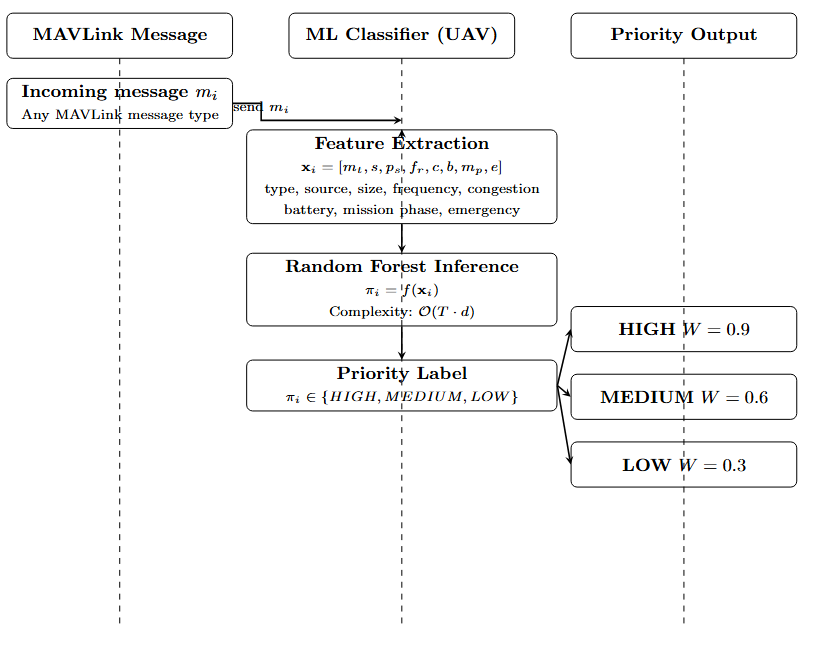
\includegraphics[width=0.85\textwidth]{chapters/flowchart_MLandCongestion.png}
\caption{ML Model and Congestion Control Flowchart}
\label{fig:flowchart_ml_congestion}
\end{figure}